\documentclass[a4paper, 12pt]{article} %--< dokumento nustatymai >--%
%\usepackage[T1]{fontenc} %--< reikia kuomet norima naudoti komanda \k{a} - a raide bus parasyta su nosine >--%
\usepackage{graphicx} %--< reikalinga paveiksliuku ikelimui >--%
\usepackage[left=1.18in,top=0.79in,right=0.39in,bottom=0.79in]{geometry} %--< parasciu nustatymai >--%
\usepackage{color} %--< spalvoto srifto nustatymai >--%
\usepackage{xcolor}
\usepackage{setspace} %--< setspace.sty failas turi buti toje pacioje direktorijoje kaip ir winedt failas >--%
\usepackage{caption} %--< leidzia rasyti komentarus po objektais >--%
\usepackage{cite} %-< reikalinga citavimui >--%
\usepackage{verbatim} %--< leidzia naudoti \begin{comment}...\end{comment} funkcijas>--%

\usepackage[utf8]{inputenc} %--< kad butu galima rasyti lietuviskai >--%
\usepackage[L7x]{fontenc}
\usepackage[lithuanian]{babel}
\usepackage{lmodern}

%\usepackage[english]{babel}
\usepackage{array}
\usepackage[titles]{tocloft}
\usepackage{amsmath} %--< formuliu rasymui >--%
\usepackage{indentfirst} %--< pirmas paragrafas prasideda su tab'u >--%
\usepackage{enumitem} %--< tarpu tarp eiluciu sarase redagavimui >--%
%\usepackage{numline} %--< eiluciu numeravimas, sio paketo naudojimas panaikina section pavadinimus >--%
\usepackage{xfrac}
\usepackage{float}
\usepackage{array}
\usepackage{multirow}
\usepackage[]{SIunits}


\makeatletter
\let\c@lofdepth\relax
\let\c@lotdepth\relax
\makeatother
\usepackage{subfigure}
%\usepackage{biblatex}

\setlength{\cftaftertoctitleskip}{-10pt}
\setlength{\cftbeforetoctitleskip}{-10pt}
%\setlength{\parskip}{6pt} %--< kiek tekstas nutoles nuo paragrafo pavadinimo >--%
\parindent=36pt %--< tab'o dydis 1 inch = 72 pt >--%

%-----------< kaip atrodo paveiksleliu ir lenteliu tesktas >-----------------%
\DeclareCaptionLabelFormat{numbfirst}{#2\bothIfSecond{\nobreakspace}{pav}} % -< paveiksliukai vadinami "pav" >- %
\DeclareCaptionLabelFormat{numbtwo}{#2\bothIfSecond{\nobreakspace}{lentel\.{e}}} % -< lenteles vadinamos "lentele" >- %
\DeclareCaptionLabelSeparator{tarpas}{. } % -< po pav taskas ir tarpas >- %
\captionsetup{justification=centering, font=normalsize, labelfont={}, textfont={it}}



%-----------------------------< keletas naudingu komandu >------------------------------------------%
\begin{comment}

-----< Lietuviskos raides, jei neveikia rasymas lietuviskai >--------
\k{a} = ą
\v{z} = ž
\v{s} = š
\.{e} = ė 
\k{e} = ę
\={u} = ū
\k{u} = ų
\k{i} = į
\v{c} = č
----------------------------------------

\textbf{padaro teksta bold}
\textit{Padaro teksta italic}
%\cite{ka cituojam}
\newpage naujas puslapis

Jei norim tekste formuliu rasom ja tarp $formule$, jei numeruotai, tai pagal
\begin{equation}
formule
label{formules_label}
\end{equation}
ir naudojam formules citavimui \ref{formule_label}

\noindent pritaukia eilute prie krasto

-------< paveiksliukams patogu susikurti atskira folderi takim paveiksliukai ar pav >--------
-------< vienas paveiksliukas >---------
\begin{figure}[H] %--< nustatymai kur bus paveiksliukas h - kaip tekste, t - puslapio virsuje, b - puslapio apacioje, H - tiksliai kaip tekste, p - atskiram paveiksleliu pslapy >--%
\centering %--< lygiavimas >--%
\includegraphics[scale=0.44]{pav/SPP_dispersijos_kreive} %--< scale - dydis, {aplankas/pav.pavadinimas} >--%
\captionsetup{labelformat=numbfirst} %--< pries tai apibrezem kaip turi atrodyti tekstas po paveiksleliu >--%
 \captionsetup{labelseparator=tarpas}
 \caption{Tesktas po paveiksleliu}
 \label{vienas}
 \end{figure}

-------< du paveiksliukai ir t.t. >---------
\begin{figure}[h]
\centering
\subfigure[]{ %--< pirmas paveiksliukas, jei [] tusti tai numeruojama raidemis >--%
\includegraphics[scale=0.3]{pav/pirmas}
\label{pirmas}
}
\centering
\subfigure[]{ %--< antras paveiksliukas >--%
\includegraphics[scale=0.27]{antras}
 \label{antras}
 }
\captionsetup{labelformat=numbfirst}
\captionsetup{labelseparator=tarpas}
\caption{Kas paveikslikuose (a) ir (b), tesktas po paveiksliuku}
\label{dupaveiksliukai}
\end{figure}

----------< numeruojam teksta >-------
\begin{enumerate}[itemsep=12pt, parsep=-10pt]
 \item[a)]  %--< jei [] nieko arba be [], tai numeruos skaiciais
\item[b)] 
\item[c)]      
\end{enumerate}

\end{comment}

%=================================================================%
%--< dalis kuria reikia uzpildyti, bet tam tikrais atvejais gali tekti pagal poreikius paredaguoti title.tex faila >--%
%=================================================================%

\newcommand{\studentas}{Mindaugas Kurmauskas} %--< cia irasyti savo varda pavarde (toliau kitus duomenis) ir nebereikes tekste >--%
\newcommand{\vadovas}{dr. Mindaugas Vil\={u}nas}
\newcommand{\recenzentas}{dr. Recenzentas}
\newcommand{\vedejas}{dr.(HP) K\k{e}stutis Arlauskas}
\newcommand{\pavadinimas}{Cortex R4 architekt\={u}ros mikrovaldiklio savybi\k{u} tyrimas} %--< cia irasyti darbo pavadinima >--%

\newcommand{\katedra}{\kkek} %--< irasyti savo, nebutinai komanda >--%
%=======%
\newcommand{\kkek}{Kieto k\={u}no elektronikos katedra}
\newcommand{\kek}{Kvantin\.{e}s elektronikos katedra}
\newcommand{\pfk}{Puslaidininki\k{u} fizikos katedra}
\newcommand{\rfk}{Radiofizikos katedra}
\newcommand{\tfk}{Teorin\.{e}s fizikos katedra}
\newcommand{\bfsk}{Bendrosios fizikos ir spektroskopijos katedra}
%==========%

\newcommand{\darbas}{\bakis} %--< irasyti savo >--%
%=========%
\newcommand{\bakikurs}{Pagrindini\k{u} studij\k{u} kursinis darbas}
\newcommand{\bakis}{Pagrindini\k{u} studij\k{u} baigiamasis darbas}
\newcommand{\magikurs}{Magistrant\={u}ros studij\k{u} kursinis darbas}
\newcommand{\magis}{Magistrant\={u}ros studij\k{u} baigiamasis darbas}
%==========%

\newcommand{\studprog}{\tf} %--< irasyti savo, nebutinai komanda >--%
%==========%
%--< besimokantiems fizfake studiju programos >--%
\newcommand{\fiz}{Fizika}
\newcommand{\tf}{Taikomoji fizika}
\newcommand{\tfe}{Telekomunikacij\={u} fizika ir elektronika}
\newcommand{\kf}{Kompiuterin\.{e} fizika}
\newcommand{\mtfv}{Moderni\k{u}j\k{u} technologij\k{u} fizika ir vadyba}
\newcommand{\bef}{Branduolin\.{e}s energetikos fizika}
\newcommand{\apchef}{Aplinkos ir chemin\.{e} fizika}
\newcommand{\bio}{Biofizika}
\newcommand{\laztech}{Lazerin\.{e}s technologijos}
\newcommand{\fiztech}{Fizikin\.{e}s technologijos ir j\k{u} vadyba}
\newcommand{\lazfiz}{Lazerin\.{e} fizika ir optin\.{e}s technologijos}
\newcommand{\mpf}{Med\v{z}iagotyra ir puslaidininki\k{u} fizika}
\newcommand{\optel}{Optoelektronikos med\v{z}iagos ir technologijos}
\newcommand{\tfem}{Telekomunikacij\k{u} fizika ir elektronika}
\newcommand{\tfa}{Teorin\.{e} fizika ir astrofizika}
%=================================================================%
%=================================================================%


%--------------------------------------< nuo cia prasideda dokumento tekstas >-------------------------------------%


\begin{document} % visas tekstas turi buti tarp begin{document} ir end{document} komandu


\begin{titlepage}

\begin{center}


% Upper part of the page

\MakeUppercase{\normalsize \textbf{Vilniaus universitetas}}\\
\MakeUppercase{\normalsize \textbf{Matematikos ir informatikos fakultetas}}\\
\MakeUppercase{\normalsize \textbf{\katedra}}\\[180pt]
%\normalsize \studentas \\ [24pt]

% Title

\MakeUppercase{{ \normalsize \pavadinimas}}\\[24pt]
\MakeUppercase{{ \normalsize \engpavadinimas}}\\[24pt]

\normalsize \darbas \\ [24pt]
(studij\k{u} programa -- \MakeUppercase{\normalsize \studprog)}\\ [130pt]

\linespread{1.3}
% Author and supervisor
\begin{minipage}{0.7\textwidth}
\begin{flushleft} \normalsize

Studentas \\  %--< nekeiciam >--%
Darbo vadovas \\ %--< nekeiciam >--%
Recenzentas\\ %--< nekeiciam >--%
\end{flushleft}
\end{minipage}
\begin{minipage}{0.29\textwidth}
\begin{flushleft} \normalsize
\studentas \\
\vadovas \\
\recenzentas \\
\end{flushleft}
\end{minipage}

\vfill

% Bottom of the page
{\normalsize Vilnius \the\year}

\end{center}

\end{titlepage}  % itraukiam titulini lapa i visa dokumenta

\newpage

\pagenumbering{arabic}
\setcounter{page}{2} % nuo kurio skaitmens pradeda numeruoti puslapius

%\tocloftpagestyle{abbrv}
\renewcommand{\cftsecleader}{\cftdotfill{\cftdotsep}} % turinio isvaizdos koregavimas

\renewcommand{\multirowsetup}{\centering}

\renewcommand{\contentsname}{Turinys}
\renewcommand\refname{Literat\={u}ros s\k{a}ra\v{s}as} % pakeicia "references" i "literaturos sarasas"
\tableofcontents

\newpage

\begin{onehalfspacing}

\section*{\k{I}vadas} % * nurodo nenumeruoti sitos dalies

\addcontentsline{toc}{section}{\k{I}vadas} % prideda prie turinio

Egzistuoja daug u\v{z}duo\v{c}i\k{u} kurioms atlikti reikia didelio patikimumo. J\k{u} atlikimui galima naudoti standartinius mikrovaldiklius, kombinuojant su programin\.emiais sprendimais. Tokiais kaip WDT $($watchdog timer$)$, kuris pri\v{z}i\=uri pagrindin\k{e} program\k{a}, kad ji tinkamai atlikt\k{u} savo darb\k{a}. Nuolatiniais testais patikrinti duomen\k{u} skai\v{c}iavimo patikimum\k{a}, pavyzd\v{z}iui atlikti algoritm\k{a} du kartus ir tikrinti ar atsakymai sutampa. Daugeliu atveju visos papildomos priemon\.es u\v{z}tikrinti patikimum\k{a} prailgina duomen\k{u} skai\v{c}iavimo laik\k{a}. \\
\indent Sistemose kurioms reikalingas didelis patikimumas ir darbas realeame laike labai praver\v{c}ia sistemos dubliavimas su tikrinimo funkcijomis. Klaidos tikimyb\.e ne visais atvejais yra tolydi laike, taigi klaidos gali tuo pa\v{c}iu metu ivykti abiejose sistemose. Tokiu atveju naudinga, kai sistemos dirba pastumtos laike at\v{z}vilgiu viena kitos. \\
\indent Yra daug aplink\k{u} kur gali reik\.eti toki\k{u} sistem\k{u}. Pramonin\.es saugumo reikalaujan\v{c}ios aplinkos, tokios kaip:
\begin{itemize}
\item automobil\k{u} stabdymo sistemos, tokios kaip rat\k{u} anti blokavimo sistema $($ABS$)$
\item elektros gaminimo ir paskirstymo sistemos.  
\item liftai ir eskalatoriai
\end{itemize}      
Medicinoje:
\begin{itemize}
\item defibriliatoriai
\item radiacijos terapija
\item robotizuotos operacijos
\end{itemize}
\noindent 
\indent Atsi\v{z}velgiant \k{i} \v{s}\k{i} poreik\k{i} kompanija
 Teksas Instruments neseniai i\v{s}leido ARM Cortex-R4 mikrovaldikli\k{u} \v{s}eim\k{a} 
 kodiniu pavadinimu Hercules. Mums kilo klausimas koks yra \v{s}i\k{u}
  mikrovaldikli\k{u} energetinis efektyvumas, bei mikrovaldikli\k{u} veikimas esant ekstramaliam poveikiui, k\k{a} \v{s}iame
   darba ir bandoma i\v{s}siai\v{s}kinti. \\
%\indent Tolimesniame darbe b\=ut\k{u} idomu patikrinti veikim\k{a} esant ekstremaliam poveikui, galimyb\k{e} panaudoti vien\k{a} i\v{s} Hercules \v{s}eimos atstov\k{u} RM48 kosmose, kur jo u\v{z}duotis gal\.et\k{u} b\=uti navigacija, kuriai atlikti reikia slankaus formato ir skai\v{c}i\k{u} tikslumo.  %

\newpage

\section{Naudojamos \k{i}rangos ir programos}
Naudojamas TMDXRM48USB maketas. Jame yra:
\begin{itemize}
\item Mikrovaldiklis xRM48L950AZWTT:
\begin{itemize}
\item Du 32-bitu ARM Cortex-R4F procesoriai, veikiantys kartu\footnote{lockstep - kartu atlieka tas pa\v{c}ias komandas}
\item 3MB flash, 256kB RAM
\item \v{S}erdies taktinis da\v{z}nis 200MHz
\item neslankaus(32bitu) ir dvigubo tikslumo (64bitu) slankaus kablelio aritmetikos modulis
\end{itemize} 
\item Integruotas XDS100v2 emuliatorius programavimui per usb
\item LED'ai, temperat\=uros sensorius, \v{s}viesos sensorius, akselerometras
\end{itemize}
Palyginimui pasirinktas STM32F4DISCOVERY maketas. Jis pasirinktas d\.{e}l 
\begin{itemize}
\item mikrovaldiklis STM32F407VGT:
\begin{itemize}
\item 32-bitu ARM Cortex-M4F procesorius
\item 1MB flash, 192 kB RAM 
\item greitis iki 168MHz 
\item neslankaus (32bitu) ir slankaus (32bitu) kablelio aritmetikos modulis
\end{itemize}
\item Integruotas ST-LINK/V2 emuliatorius programavimui per usb
\item LED'ai, akselerometras, skaitmeninis mikrofonas
\item CS43L22- SAK garsui su integruotu D klas\.es garso stiprinimu
\end{itemize}
Pasirinktas kompiliatorius - IAR 6.4. Darbo prad\.ejimo metu vienintelis palaik\.e abu maketus be papildomos \k{i}rangos. 
\subsection{xRM48L950 apra\v{s}as}
 
\subsubsection{Procesorius}
xRM48L950 turi dvi integruotas 32-bit\k{u} RISC ARM Cortex-R4F \v{s}erdis, su slankaus kablelio aritmetikos moduliu. \v{S}erdys i\v{s}destyti skirtinga orientacija  
\begin{figure}[H] %--< nustatymai kur bus paveiksliukas h - kaip tekste, t - puslapio virsuje, b - puslapio apacioje, H - tiksliai kaip tekste, p - atskiram paveiksleliu pslapy >--%
\centering %--< lygiavimas >--%
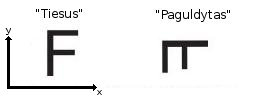
\includegraphics[scale=2.5]{pav/orentacija.jpg} %--< scale - dydis, {aplankas/pav.pavadinimas} >--%
\captionsetup{labelformat=numbfirst} %--< pries tai apibrezem kaip turi atrodyti tekstas po paveiksleliu >--%
\captionsetup{labelseparator=tarpas}
\caption{\v{S}erdys pakreipitos fizi\v{s}kai viena kitos at\v{z}vilgiu korpuse}
\label{vienas}
\end{figure}

Taip pat taktinis da\v{z}nis procesoriams paduodamas su 2 takt\k{u} u\v{z}laikymo skirtumu. Procesoriai fizi\v{s}kai atskirti 100$\micro$m. atstumu.  
Procesori\k{u} i\v{s}\.ejimo signalai palyginami atskirame modulyje.
\begin{figure}[H] %--< nustatymai kur bus paveiksliukas h - kaip tekste, t - puslapio virsuje, b - puslapio apacioje, H - tiksliai kaip tekste, p - atskiram paveiksleliu pslapy >--%
\centering %--< lygiavimas >--%
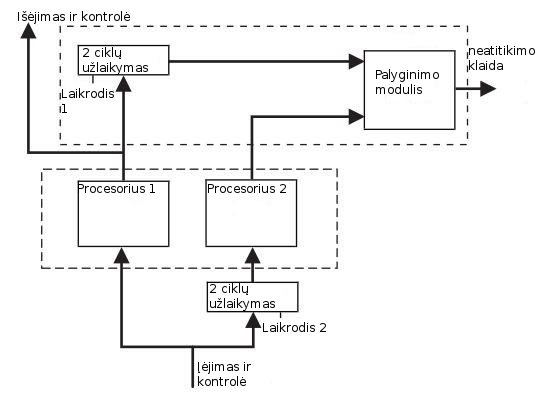
\includegraphics[scale=2.8]{pav/impl.jpg} %--< scale - dydis, {aplankas/pav.pavadinimas} >--%
\captionsetup{labelformat=numbfirst} %--< pries tai apibrezem kaip turi atrodyti tekstas po paveiksleliu >--%
\captionsetup{labelseparator=tarpas}
\caption{Dviej\k{u} branduoli\k{u} \k{i}gyvendinimas}
\label{vienas}
\end{figure}
\k{I}renginys palaiko sav\k{e}s testavim\k{a}. Jo metu galima priversti procesori\k{u} i\v{s}\.ejimo signal\k{u} nesutapim\k{a}, taip patikrinama ar veikia procesori\k{u} palyginimo modulis ir ar \k{i}renginys sugeba atpa\v{z}inti klaidas. Procesoriai maitinami 1.2V \k{i}tampa. 


\subsubsection{Atmintys}
\k{I}renginys palaiko little-endian $($LE32$)$ format\k{a}. Tai rei\v{s}kia, kad atmintyje jauniausias bitas yra saugomas pirmas.
SRAM ir Flash atminys turi ECC\footnote{ECC - error corection code} apsaug\k{a} - galimyb\.e 1 bito klaidos aptikimui ir pataisymui, bei 2 bit\k{u} klaidos aptikimui 8bit\k{u} bloke. Flash atmintis maitinama 3.3V \k{i}tampa. Esant kaskadiniui
re\v{z}imui flash atmintis gali veikti iki 200MHz taktiniu da\v{z}niu. SRAM atmint\k{i} galima nuskaityti arba ira\v{s}yti 1 ciklu nepriklausomai nuo re\v{z}imo.   


\subsubsection{Tr\=uki\k{u} sistema}
Vektorinis tr\=uki\k{u} valdiklis \k{i}galina veiksm\k{u} prioritizavim\k{a} ir kontrol\k{e}. Tr\=ukis - tai paprogram\.es i\v{s}kvietimas, galimai nutraukiant esam\k{a} procesoriaus veikl\k{a}. Paprastai toks \k{i}vykis reikalauja greito procesoriaus atsako. Procesorius i\v{s} normalios programos per\v{s}oka \k{i} tr\=ukio aptarnavimo paprogram\k{e}. RM48 palaiko 96 skirtingus programi\v{s}kai reguliuojamo prioriteto tr\=ukius. Yra 2 tr\=ukio vektoriai - normal\=us tr\=ukiai $($IRQ\footnote{IRQ - interrupt request}$)$ ir greitieji tr\=ukiai $($FIQ\footnote{FIQ - fast interrupt request}$)$. Greitieji tr\=ukiai turi didesn\k{i} prioriteta u\v{z} normalius ir yra nemaskuojami t.y. juos \k{i}jungus j\k{u} neimanoma i\v{s}jungti ar pakeisti, nebent atlikus sistemos perkrovima, kai visi tr\=ukiai yra automati\v{s}kai i\v{s}jungiami. Greitieji tr\=ukiai gali pertraukti normalius.  


\subsubsection{Prievadai}
RM48L950 turi 2 laikma\v{c}i\k{u} $($N2HET\footnote{N2HET - next generation high end timer}$)$ koprocesorius su tiesiogine magistrales prieiga $($DMA$)$ realaus laiko kontrolei. J\k{u} pagalba galima atlikti \v{i}tampos impulso plo\v{c}io moduliacij\k{a} $($PWM$)$, steb\.eti i\v{s}vado login\k{i} lyg\k{i}, bei gali veikti kaip \k{i}vesties/i\v{s}vesties periferija. Taipat yra du integruoti 12 bit\k{u} rezoliucijos analogas kodas keitikliai. Prievadai maitinami 3.3V \k{i}tampa. Taipat yra bendrosios paskirties \k{i}vesties i\v{v}esties prievadai.
Palaiko \v{s}ias periferijas:
\begin{itemize}
\item USB
\item Ethernet
\item UART
\item MibSPI
\item $I^2C$
\item SCI
\item DCAN
\end{itemize}



\subsection{STM32F4 apra\v{s}as}


\subsubsection{Procesorius}
ARM Cortex-M4F 32-bit\k{u} RISC procesorius, su slankaus kablelio aritmetikos moduliu. Palaiko DSP instrukcijas ir 32bit\k{u} slankaus kablelio duomenis.      


\subsubsection{Atmintys}
Adaptyvus realaus laiko atminties greitintuvas leid\v{z}ia minimal\k{u} procesoriaus laukim\k{a} esant dideliems taktavimo da\v{z}niams nuskaitant ir \k{i}ra\v{s}ant \k{i} Flash atmint\k{i}. SRAM atmintis nuskaitom ir \k{i}ra\v{s}oma per 1 takt\k{a}. Atminties apsaugos modulis riboja procesoriaus pri\.ejim\k{a} prie atminties, kad b\=ut\k{u} galima i\v{s}vengti nety\v{c}ini\k{u} atminties sugadinim\k{u}. Tai ypa\v{c} praver\v{c}ia kai turima kriti\v{s}kai svarbi\k{u} duomen\k{u} ir juos reikia apsaugoti nuo kit\k{u} veikian\v{c}i\k{u} proces\k{u}. Pavyzd\v{z}iui, jeigu yra veikianti operacin\.e sistema procesoriuje.


\subsubsection{Tr\=uki\k{u} sistema}
Palaiko \k{i}d\.etin\k{e} vektorin\k{e} tr\=uki\k{u} kontrol\k{e} $($NVIC\footnote{NVIC - nested vectored interrupt controller}$)$.
Yra 16 prioritet\k{u} lygi\k{u}, 82 maskuojami tr\=uki\k{u} kanalai. Leid\v{z}ia auk\v{s}tesnio prioriteto tr\=ukiams pertraukti vykdomus \v{z}emesnio prioriteto tr\=ukius, minimaliai apkraunant procesori\k{u}. 


\subsubsection{Prievadai}    
140 \k{i}\.ejimo i\v{s}\.ejimo bendrosios paskirties prievad\k{u}, su tr\=ukio generavimo galimybe. Periferijos greitis - iki 84MHz. Du 12 bit\k{u} skaitmeninis analogas keitikliai. Trys 12 bit\k{u} analogas kodas keitikliai. 
Palaikomos periferijos:
\begin{itemize}
\item $I^2C$
\item SPI
\item UART
\item $I^2S$
\item CAN
\item USB 2.0
\item Ethernet
\end{itemize}

\newpage %perkelia testa i nauja lapa
\section{Ka kas ir kaip}
%%%%%%%%%%%%%%%%%%%%%%%%%%%%%%%%%%%%%%%%%%%%%%%%%%%%
%
%%%%%%%%%%%%%%%%%%%%%%%%%%%%%%%%%%%%%%%%%%%%%%%%%%%%
\section{Naudoti testavimo algoritmai ir j\k{u} apra\v{s}ai}
%\addcontentsline{toc}{section}{Praktin\.{e}\ dalis} % prideda
\subsection{Matematini\k{u} funkcij\k{u} skai\v{c}iavimo grei\v{c}i\k{u} \k{i}vertinimo algoritmai}
\v{S}iame paragrafe apra\v{s}ytiems algoritmams buvo naudojamas laiko tr\=ukis, kurio pagalba buvo ska\v{c}iuojamas algoritmo atlikimo greitis 1ms tikslumu. Abu maketai buvo nustatyti veikti 100MHz grei\v{c}iu. Algoritmai buvo leisti 100 kart\k{u} ir fiksuoti u\v{z}duoties atlikimo laikai suvidurkinti.
\subsubsection{Slankaus kablelio algoritmai}
Slankaus kablelio Gauss Legendre algoritmas $\pi$ skai\v{c}iavimui:
\begin{equation*}\label{xx}
a_{0}=1\;b_{0}=\frac{1}{\sqrt{2}}\;t_{0}=\frac{1}{4}\;p_{0}=1\\
\end{equation*}
\begin{equation*}
a_{n+1} = \frac{a_n + b_n}{2},
\end{equation*}
\begin{equation*}
b_{n+1} = \sqrt{a_n b_n}, 
\end{equation*}
\begin{equation*}
t_{n+1} = t_n - p_n(a_n - a_{n+1})^2, 
\end{equation*}
\begin{equation*}
p_{n+1} = 2p_n. 
\end{equation*}
\begin{equation}
\pi \approx \frac{(a_n+b_n)^2}{4t_n}
\end{equation}
Naudojant dvigubo tikslumo kintam\k{u}j\k{u} test\k{a} buvo ie\v{s}komas 1000 narys, suskai\v{c}iuota  
konstanta nuo pasirinktosios skiriasi $3.55271 * 10^{-15}$. 
%\textcolor{gray}{\\
\begin{verbatim}
  int doubleTest() { 
    volatile int i; 
    volatile double an,bn,tn,pi; 
    volatile double a,b,t,p;  
    a = 1.0; b = 1/sqrt(2); 
    t = 1/4; p = 1.0; 
    for (i = 0; i < 1000; i++) { 
      an = (a+b)/2;  
      bn = sqrt(a*b); 
      tn = t - p*(a-an)*(a-an);  
      p *= 2; 
      pi = (an+bn)*(an+bn)/(4*tn);  
      a = an; b = bn; t = tn; 
    }
    if ((pi - 3.14159265358979) <= 3.55271e-15) 
      return 1; //testas atliktas sekmingai
    return 0;  //teste ivyko klaida
  } 
\end{verbatim}
%}
Naudojant viengubo tikslumo slankaus kablelio kintamuosius buvo ie\v{s}komas 120 narys. Konstanta nuo pasirinktosios skiriasi $8.74228* 10^{-8}$
\begin{verbatim}
int floatTest() {
  volatile int i;
  volatile float an,bn,tn,pi;
  volatile float a,b,t,p;
  for(volatile int j = 0; j <9; j++) {
    a = 1.0; b = sqrt(0.5);
    t = 0.25; p = 1.0;
    for (i = 0; i < 120; i++) {
      an = (a+b)/2;
      bn = sqrt(a*b);
      tn = t - (p*(a-an)*(a-an));
      p *= 2;
      pi = (an+bn)*(an+bn)/(4*tn);
      a = an; b = bn; t = tn;
    } 
  }
  if ((pi - 3.14159265358979) <= 8.74228e-8)
    return 1; //testas atliktas sekmingai
  return 0; //teste ivyko klaida
}
\end{verbatim}
\subsubsection{Fiksuoto tikslumo algoritmas}
Fiksuoto tikslumo algoritmas:
\begin{equation}
b = \sum_{i=0}^{100000} (i * (-1)^{i+1})
\end{equation}

\begin{verbatim}
void intTest() {
  volatile int a,b;
  a = 1;
  b = 0;
  for(volatile int i = 0; i < 100000; i++) {
    b += i * a;
    a *= -1;
  }
}
\end{verbatim}
\subsubsection{Logini\k{u} funkcij\k{u} testavimo algoritmas}
Mikrovaldikliai atlieka logines AND, NOT, OR, XOR, bei bit\k{u} stumdymo funkcijas. 
\begin{verbatim}
short testBits() {
  volatile unsigned sum = 0x55555555; 
  // 0101 0101  0101 0101  0101 0101  0101 0101  
  for (volatile int i = 0; i < 0x020000; i++) {
    sum = sum << 1;          /// sum = 0xAAAAAAAA 
    sum &= 0x0000FFFF;       /// sum = 0x0000AAAA
    sum ^= 0xFFFFFFFF;       /// sum = 0xFFFF5555
    sum = sum << 16;         /// sum = 0x55550000
    sum = sum | (sum >> 16); /// sum = 0X55555555
    sum = ~sum;              /// sum = 0xAAAAAAAA
    sum = sum >> 1;          /// sum = 0x55555555
  }
  if (0x55555555 == sum)
    return 1; //testas ivykditas sekmingai
  return 0; // teste ivyko klaida
}
\end{verbatim}
\subsubsection{Greitas disckretinis Furj\.e\ eilut\.es transformavimo testas}
Naudotos ARM dsp\footnote{Dsp - digital signal processing $($skaitmeninis signal\k{u} apdorojimas$)$} bibliotekos, atskirai optimizuotos R4 bei M4 mikrovaldikliams. Naudota 1024 kompleksini\k{u} ta\v{s}k\k{u}, kurie masyve i\v{s}d\.estyti vienas po kito ir bendras masyvo ilgis 2048. Slankaus kablelio testui masyvas u\v{z}pildomas funkcija:
\begin{equation*}
Re(z) = (sin(v*i) + cos(v*7)),\; t = 0, 2, 4... 2046
\end{equation*}
\begin{equation}
Im(z) = 0
\end{equation}
\begin{verbatim}
#define TEST_LENGTH_SAMPLES 2048 
static float32_t testInput[TEST_LENGTH_SAMPLES]; 
static float32_t testOutput[TEST_LENGTH_SAMPLES/2]; 
uint32_t fftSize = 1024; 
uint32_t ifftFlag = 0; 
uint32_t doBitReverse = 1; 

void prepareTestFloat(void) {
  for(volatile int t = 0; t < 2048; t+=2) {
    testInput[i] = sin(t*3) + cos(t*7);
    testInput[i+1] = 0;
  }
}

int32_t testCfftFloat(void) { 
  arm_status status; 
  arm_cfft_radix4_instance_f32 S; 
  float32_t maxValue;  
   
  arm_cfft_radix4_init_f32(&S, fftSize, ifftFlag, doBitReverse); 
   
  arm_cfft_radix4_f32(&S, testInput); 
   
  arm_cmplx_mag_f32(testInput, testOutput, fftSize);  
   
  arm_max_f32(testOutput, fftSize, &maxValue, &testIndex); 
   
  if(testIndex == refIndex) { 
    return 1;
  }
  return 0;
} 
\end{verbatim}  
Fiksuoto tikslumo Furij\.e transformacijai naudoti ARM Q31 fiksuoto kablelio kintamieji. I\v{s} slankaus kablelio paversti \k{i} Q31 formato kintamuosius naudota funkcija:
\begin{equation}
Q31(x)= ((int)\; ((x)*(float)(1<<31))\; )
\end{equation}   
Masyvo u\v{z}pildo funkcija:
\begin{equation*}
Re(z) = Q31(1000*(sin(v*i) + cos(v*7)))),\; t = 0, 2, 4... 2046
\end{equation*}
\begin{equation}
Im(z) = 0
\end{equation}
\begin{verbatim}
#define TEST_LENGTH_SAMPLES 2048
uint32_t fftSize = 1024; 
uint32_t ifftFlag = 0; 
uint32_t doBitReverse = 1; 
static q31_t testInputQ[TEST_LENGTH_SAMPLES]; 
static q31_t testOutputQ[TEST_LENGTH_SAMPLES/2]; 
uint32_t refQIndex = 0;

void prepareTestQ31(void) {
  double skaicius=0;
  int nulis = (int) ((0 * (float)(1<<31)));
  for(volatile int32_t i = 0; i < 2048; i+=2) {
    skaicius = 1000*sin(i*3) + 1000*cos(i*7);
    testInputQ[i] = ((int)(skaicius * (float)(1<<31)));
    testInputQ[i+1] = nulis;
  }
}

int32_t testCfftQ31(void) { 
  arm_status status; 
  arm_cfft_radix4_instance_q31 S; 
  q31_t maxValue; 
   
  status = arm_cfft_radix4_init_q31(&S, fftSize, ifftFlag, doBitReverse); 
   
  arm_cfft_radix4_q31(&S, testInputQ); 
  
  arm_cmplx_mag_q31(testInputQ, testOutputQ, fftSize);  
 
  arm_max_q31(testOutputQ, fftSize, &maxValue, &testIndex); 

  if(testIndex == refIndex) { 
    return 1;
  } 
  return 0;
}
\end{verbatim}
\subsection{\k{I}\.ejimo ir i\v{s}\.ejimo \k{i} tr\=uk\k{i} algoritmo apra\v{s}ymas}
Naudojami maketai buvo paleisti veikti 100MHz grei\v{c}iu. Abu maketai keisdavo i\v{s}\.ejimo prievado vieno i\v{s} i\v{s}vad\k{u} login\k{i} lyg\k{i}, bei buvo \k{i}jungtas taimeris su tu\v{s}\v{c}ia paprograme. Osciloscopu matuotas i\v{s}vad\k{u} lygmen\k{u} kitimo laikas.
\subsection{Srov\.es matavimai}
STM32F4DISCOVERY makete srov\.e matuota tiesiogiai. TMDXRM48USB maketas netur\.ejo 
trumpikli\k{u} tarp maitinimo ir mikrovaldiklio. Tarp maitinimo 3.3V i\v{s}\.ejimo ir mikrovaldiklio i\v{s}vad\k{u} maitinimo bei maitinimo 1.2V i\v{s}\.ejimo ir mikrovaldiklio logikos maitinimo buvo \k{i}terptos 0.12$\Omega$ var\v{z}os. 
\begin{figure}[H] %--< nustatymai kur bus paveiksliukas h - kaip tekste, t - puslapio virsuje, b - puslapio apacioje, H - tiksliai kaip tekste, p - atskiram paveiksleliu pslapy >--%
\centering %--< lygiavimas >--%
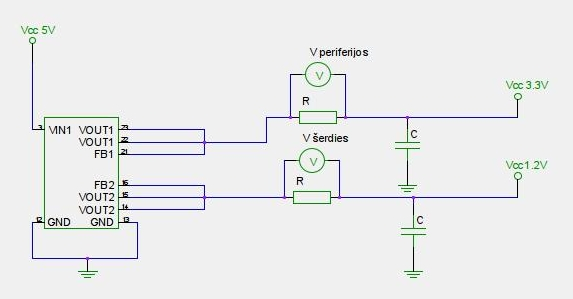
\includegraphics[scale=0.8]{pav/srovesc.jpeg} %--< scale - dydis, {aplankas/pav.pavadinimas} >--%
\captionsetup{labelformat=numbfirst} %--< pries tai apibrezem kaip turi atrodyti tekstas po paveiksleliu >--%
\captionsetup{labelseparator=tarpas}
\caption{Cortex-R4 srov\.{e}s matavimo schema. R=0.12 $\Omega$.}
\label{vienas}
\end{figure}
Vis\k{u} matavim\k{u} metu 
  i\v{s}vadai buvo nustatyti i\v{s}vesties re\v{z}ime ir 
  nustatyti nuliniame loginiame lygije. Buvo atlikti matavimai
  esant \v{s}ioms konfig\={u}racijoms:
\begin{itemize}
\item \k{i}jungtas stanby re\v{z}imas. Siekta i\v{s}matuoti minimal\k{u} srov\.{e}s sunaudojim\k{a} kai procesoriui nereikia atlikti darbo. 
\begin{itemize} 
\item Cortex-R4:
\begin{itemize}
\item Flash atmintis automatinio miego re\v{z}ime
\item procesoriai laukimo re\v{z}ime
\item taktuojama i\v{s} ma\v{z}os galios i\v{s}orinio kvarco 
\item periferijos i\v{s}jungtos
%damusti------------------------------------------%
\end{itemize}

\item Cortex-M4:
\begin{itemize}
\item vidinis 1.2V \k{i}tampos reguliatorius i\v{s}jungtas
\item Pll\footnote{PLL - phase lock loop da\v{z}ni\k{u} generatorius}, vidinis 16MHz ir i\v{s}orinis 8MHz taktiniai osciliatoriai atjungti. Veikia vidinis 32kHz taktinis osciliatorius
\item procesorius sustabdytas
\item mikrovaldiklis minimalioje srov\.es suvartojimo b\=usenoje.
\item re\v{z}im\k{a} galima i\v{s}eiti:
\begin{itemize} 
\item gavus i\v{s}orin\k{i} impuls\k{a} \k{i} NRST arba WKUP i\v{s}vadus 
\item realaus laiko laikrod\v{z}iui $($RTC$)$ sugeneravus tr\=uk\k{i}
\end{itemize} 
\end{itemize}
\end{itemize}
\item \k{i}jungtas negilaus miego re\v{z}imas esant \k{i}vairiems taktavimo grei\v{c}iams:
\begin{itemize} %aprasyti sleep modey
\item Cortex-R4:
\begin{itemize}
\item Flash atmintis automatinio miego re\v{z}ime
\item sistema veikia taktavimo da\v{z}niu
\item procesoriai laukimo re\v{z}ime
\item periferija atjungta
\end{itemize}
\item Cortex-M4:
\begin{itemize}
\item sistema veikia pll taktavimo da\v{z}niu
\item procesorius sustabdytas 
\item i\v{s} re\v{z}imo galima i\v{s}eiti betkokio tr\=ukio pagalba
\end{itemize}
\end{itemize}
\item esant skirtingiems taktavimo da\v{z}niams mikrovaldikliai atlikin\.ejo slankaus kablelio ir fiksuoto tikslumo aritmetikos testus, bei buvo paleisti veikti cikle: \begin{verbatim} while(1); \end{verbatim} 
\end{itemize}
\subsection{Radiacinis matavimas}
Siekiant patikrinti mikrovaldiklio veikim\k{a} ekstremaliam poveikiui. Buvo i\v{s}kelta hipotez\.{e}, kad ap\v{s}vie\v{c}iant jonizuojan\v{c}i\k{a}j\k{a} spinduliuote gali b\={u}ti sutrigdoma normali mikrovaldiklio veika:
\enumerate{itemize}
\item pa\v{z}eid\v{z}iant flash atmint\k{i} sutrigdoma programa, d\.{e}l ko mikrovaldiklis pradeda vykdyti neteisingas u\v{z}duotis arba j\k{u} i\v{s}vis nevykdyti.
\item pa\v{z}eid\v{z}iant RAM atmint\k{i} gali b\={u}ti i\v{s}kraipomi skai\v{c}iavim\k{u} duomenys
\item sutrigdant \v{s}erdies atliekam\k{a} darb\k{a} gali b\={u}ti generuojamos skai\v{c}iavim\k{u}, logikos ir valdymo klaidos.
\end{itemize} 
Cortex-M4 ir Cortex-R4 mikrovaldikliai sujungti 4 laidu + \v{z}em\.{e} spi protokolu. Cortex-M4 nustatytas kaip master, Cortex-R4 kaip slave.
Cortex-M4 atlikin\.{e}jo matematinius skai\v{c}iavimus ir siunt\.{e} rezultatus \k{i} Cortex-R4 mikrovaldikl\k{i} patikrinimui, kuris per UART jungt\k{i} juos siunt\.{e} \k{i} kompiuterio terminal\k{a}.  
\begin{figure}[H] %--< nustatymai kur bus paveiksliukas h - kaip tekste, t - puslapio virsuje, b - puslapio apacioje, H - tiksliai kaip tekste, p - atskiram paveiksleliu pslapy >--%
\centering %--< lygiavimas >--%
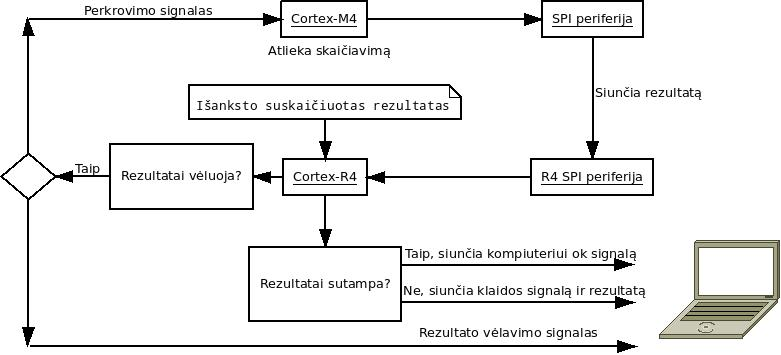
\includegraphics[scale=0.6]{pav/raddiag.jpg} %--< scale - dydis, {aplankas/pav.pavadinimas} >--%
\captionsetup{labelformat=numbfirst} %--< pries tai apibrezem kaip turi atrodyti tekstas po paveiksleliu >--%
\captionsetup{labelseparator=tarpas}
\caption{Radiacinio matavimo logikos diagrama.}
\label{vienas}
\end{figure}
%------------------------------%
\newpage
   
\section{Rezultatai}
Cortex-R4 mikrovaldiklis beveik visus skai\v{c}iavimo testus atliko grei\v{c}iau nei cortex-M4 mikrovaldiklis esant 100MHz taktiniui da\v{z}niui. 
\begin{figure}[H] %--< nustatymai kur bus paveiksliukas h - kaip tekste, t - puslapio virsuje, b - puslapio apacioje, H - tiksliai kaip tekste, p - atskiram paveiksleliu pslapy >--%
\centering %--< lygiavimas >--%
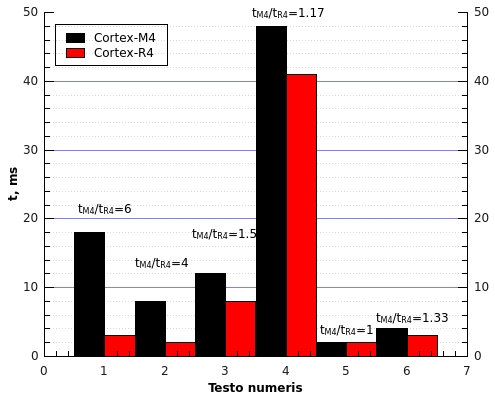
\includegraphics[scale=0.8]{pav/testai.jpg} %--< scale - dydis, {aplankas/pav.pavadinimas} >--%
\captionsetup{labelformat=numbfirst} %--< pries tai apibrezem kaip turi atrodyti tekstas po paveiksleliu >--%
\captionsetup{labelseparator=tarpas}
\caption{Skai\v{c}iavimo algoritm\k{u} laikai. 1 - dvigubo tikslumo slankaus kablelio testas $($$($2.1.1$)$ algoritmas$)$. 2 - slankaus kablelio testas $($$($2.1.1$)$ antras algoritmas$)$. 3 - fiksuoto tikslumo kintam\k{u}j\{u} testas $($$($2.1.2$)$ algoritmas$)$. 4 - logini\k{u} funkcij\k{u} testas $($$($2.1.3$)$ algoritmas$)$. 5 - Furij\.e slankaus kablelio $($$($2.1.4$)$ algoritmas$)$. 6 - Furij\.e fiksuoto tikslumo kintam\k{u}j\k{u} testas$($$($2.1.4$)$ antras algoritmas$)$.}
\label{vienas}
\end{figure}


Tirtas periferijos perjungimo greitis ir \k{i}\.ejimo i\v{s}\.ejimo i tu\v{s}\v{c}i\k{a} tr\=ukio paprogram\k{e} laikas esant 100MHz taktavimo da\v{z}niui.  
Cortex-R4 periferijos i\v{s}\.ejimo lygmen\k{i} keit\.{e} kas 280ns. \k{I}\.ejimo \k{i} tr\=uk\k{i} ir i\v{s}\.ejimo laikas 730ns. Skirtumo tarp IRQ ir FIQ tr\=uki\k{u} laiko nebuvo. Cortex-M4 periferikos i\v{s}vado login\k{i} lygmen\k{i} keit\.e kas 150ns. \k{I}\.ejimo \k{i} tr\=uk\k{i} ir i\v{s}\.ejimo laikas 200ns.
\begin{figure}[H] %--< nustatymai kur bus paveiksliukas h - kaip tekste, t - puslapio virsuje, b - puslapio apacioje, H - tiksliai kaip tekste, p - atskiram paveiksleliu pslapy >--%
\centering %--< lygiavimas >--%
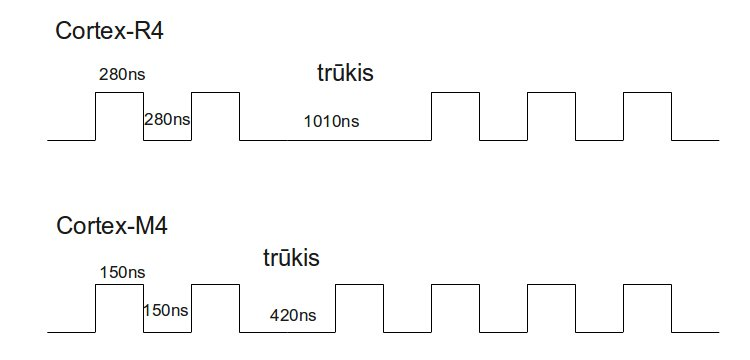
\includegraphics[scale=0.4]{pav/trukiai.jpg} %--< scale - dydis, {aplankas/pav.pavadinimas} >--%
\captionsetup{labelformat=numbfirst} %--< pries tai apibrezem kaip turi atrodyti tekstas po paveiksleliu >--%
\captionsetup{labelseparator=tarpas}
\caption{Generuot\k{u} impuls\k{u} laikin\.e diagrama.}
\label{vienas}
\end{figure}
Mikrovaldiklio Cortex-R4 periferija tirta atskirai. Maitinama 3.3V.
\begin{itemize}
\item Prievadai nustatyti \v{z}emame loginiame lygyje:
\begin{itemize}
\item Naudajama galia 371.5mW
\end{itemize}
\item Periferija i\v{s}jungta:
\begin{itemize}
\item Periferijos i\v{s}vaduose atsiranda loginis auk\v{s}tas lygis:
\begin{itemize}
\item SPI4nCS, SPI4nENA
\item DMMnENA
\item CAN3TX, CAN3RX
\end{itemize}
\item Naudojama galia 341mW
\end{itemize}
\item Nurodomas ma\v{z}os galios osciliatorius periferij\k{u} taktavimui. Periferija i\v{s}jungiama
\begin{itemize}
\item I\v{s}jungiant periferij\k{a} tur\.{e}t\k{u} b\={u}ti automati\v{s}kai atjungiami ir osciliatoriai
\item Naudojama periferijos galia 283.25mW
\item $($Procesoriaus naudojama galia minimali (4mW)$)$
\end{itemize} 
\item I\v{s}jungiamos periferijos bei procesoriaus login\.{e} dalis atsakinga u\v{z} periferijos valdym\k{a}
\begin{itemize}
\item Mikrovaldiklis nustoja vykdyti kitas komandas
\item Naudojama periferijos galia 374mW
\item Padid\.{e}ja procesoriaus naudojama galia (16mW) lyginant su prie\v{s} tai atliktu matavimu.
\end{itemize}
\end{itemize}

Mikrovaldiklio Cortex-R4 \v{s}erdis maitinama 1.2V. Kadangi 3.3V maitinama ir kiti \k{i}renginiai esantys makete $($tokie kaip \v{s}viesos sesnosrius, akselerometras$)$, bei d\.{e}l galimos JTAG \k{i}takos rezultatams naudojama galia buvo skai\v{c}iuojama pagal formul\k{e} $P=I_{serdies} *1.2V$. Cortex-M4 maitinamas 3.3V. Skai\v{c}iuojant gali\k{a} daryta prielaida, kad i\v{s}jungus periferij\k{a} kit\k{u} \k{i}rengini\k{u} naudojama srov\.{e} yra apie 0mA. Cortex-M4 naudojama galia $P=I*3.3V$.
%--------------------%
\begin{figure}[H] %--< nustatymai kur bus paveiksliukas h - kaip tekste, t - puslapio virsuje, b - puslapio apacioje, H - tiksliai kaip tekste, p - atskiram paveiksleliu pslapy >--%
\centering %--< lygiavimas >--%
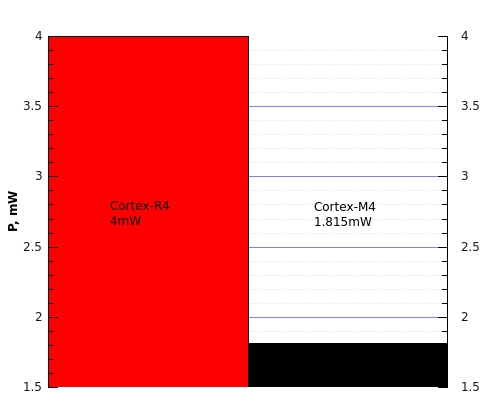
\includegraphics[scale=0.8]{pav/modes.jpg} %--< scale - dydis, {aplankas/pav.pavadinimas} >--%
\captionsetup{labelformat=numbfirst} %--< pries tai apibrezem kaip turi atrodyti tekstas po paveiksleliu >--%
\captionsetup{labelseparator=tarpas}
\caption{Mikrovaldikliai stanby re\v{z}ime.}
\label{vienas}
\end{figure}
\begin{figure}[H] %--< nustatymai kur bus paveiksliukas h - kaip tekste, t - puslapio virsuje, b - puslapio apacioje, H - tiksliai kaip tekste, p - atskiram paveiksleliu pslapy >--%
\centering %--< lygiavimas >--%
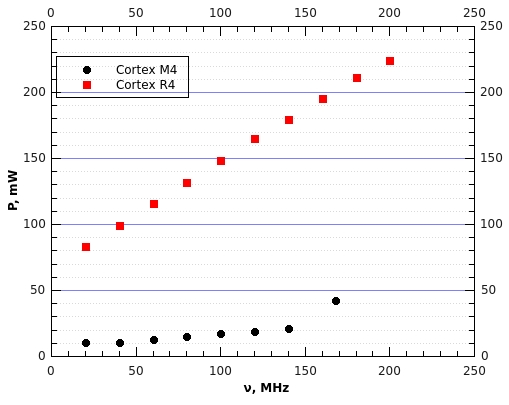
\includegraphics[scale=0.8]{pav/sleep.jpg} %--< scale - dydis, {aplankas/pav.pavadinimas} >--%
\captionsetup{labelformat=numbfirst} %--< pries tai apibrezem kaip turi atrodyti tekstas po paveiksleliu >--%
\captionsetup{labelseparator=tarpas}
\caption{Mikrovaldikli\k{u} galios vartojimo priklausomyb\.e nuo taktinio grei\v{c}io sleep re\v{z}ime.}
\label{vienas}
\end{figure}
\begin{figure}[H] %--< nustatymai kur bus paveiksliukas h - kaip tekste, t - puslapio virsuje, b - puslapio apacioje, H - tiksliai kaip tekste, p - atskiram paveiksleliu pslapy >--%
\centering %--< lygiavimas >--%
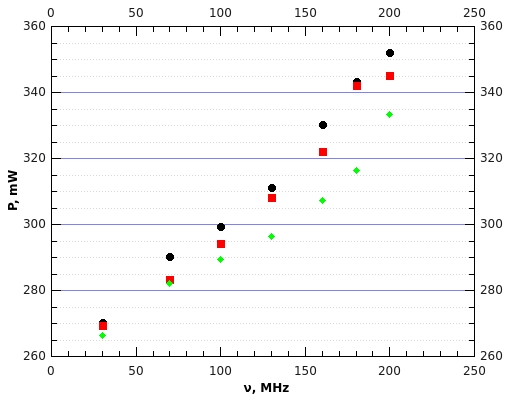
\includegraphics[scale=0.8]{pav/R4galia.jpg} %--< scale - dydis, {aplankas/pav.pavadinimas} >--%
\captionsetup{labelformat=numbfirst} %--< pries tai apibrezem kaip turi atrodyti tekstas po paveiksleliu >--%
\captionsetup{labelseparator=tarpas}
\caption{RM48 mikrovaldiklio naudojamos galios priklausomyb\.e nuo taktinio da\v{z}nio atliekant slankaus kablelio, fiksuoto tikslumo ir b\=unant tu\v{s}\v{c}iame cikle.}
\label{vienas}
\end{figure}
\begin{figure}[H] %--< nustatymai kur bus paveiksliukas h - kaip tekste, t - puslapio virsuje, b - puslapio apacioje, H - tiksliai kaip tekste, p - atskiram paveiksleliu pslapy >--%
\centering %--< lygiavimas >--%
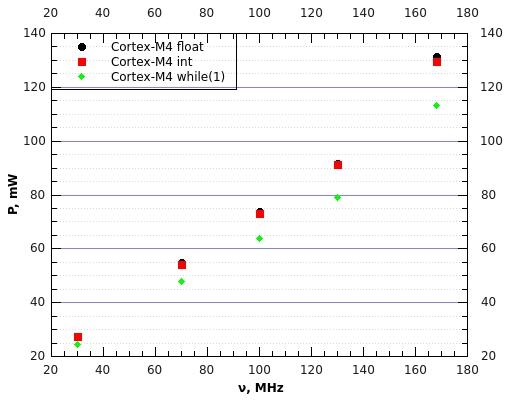
\includegraphics[scale=0.8]{pav/M4galia.jpg} %--< scale - dydis, {aplankas/pav.pavadinimas} >--%
\captionsetup{labelformat=numbfirst} %--< pries tai apibrezem kaip turi atrodyti tekstas po paveiksleliu >--%
\captionsetup{labelseparator=tarpas}
\caption{STM32F4 mikrovaldiklio naudojamos galios priklausomyb\.e nuo taktinio da\v{z}nio atliekant slankaus kablelio, neslankaus kablelio ir b\=unant tu\v{s}\v{c}iame cikle.}
\label{vienas}
\end{figure}
Mikrovaldiklis Cortex-M4 buvo 1h \v{s}vitinamas 1.176MeV gama spinduliais $($\^{137}Cs$)$. Joki\k{u} nukripim\k{u} nuo normalaus mikrovaldiklio darbo neu\v{z}fiksuota.
Pereita prie \v{s}vitinimo rentgeno spinduliuote. Mikrovaldiklis buvo pad\.{e}tas po rentgeno lempa kurios \k{i}tampa bei srov\.{e} didinta laipsni\v{s}kai. Prie 19kV \k{i}tampa ir 19mA per 15min mikrovaldiklis nustojo veikti, ta\v{c}iau iki nustojimo veikti visus skai\v{c}iavumus atliko gerai. Mikrovaldiklis per 3h atsistat\.{e} ir v\.{e}l prad\.{e}jo atlikin\.{e}ti skai\v{c}iavimus.
\newpage
\section{I\v{s}vados}


\begin{enumerate}
\item Cortex-R4, esant 100MHz taktiniui da\v{z}niui, yra \v{z}ymiai greitesnis atliekant dvigubo tikslumo slankaus kablelio skai\v{c}iavimus nei cortex-M4 mikrovaldiklis.
%\item Du procesoriai esantys R4 stipriai padidina mikrovaldiklio naudojam\k{a} gali\k{a}
%\item RM48 mikrovaldiklio periferija dirba l\.{e}\v{c}iau nei stm32f4 esant 100MHz taktiniam da\v{z}niui.
\item Cortex-R4 tr\=uki\k{u} sistema lyginant su Cortex-M4 yra labai l\.{e}ta ir neefektyvi.
%\item Ma\v{z}iausia naudojama galia, kuri\k{a} pavyko pasiekti su RM48 yra 82 kartus didesn\.e nei ma\v{z}iausia vartojama galia, kuri\k{a} pavyko pasiekti su stm32f4 maketu.%
\item Mikrovaldikliams atliekant skirtingus skai\v{c}iavimus naudojama galia labiausiai priklauso nuo taktinio da\v{z}nio ir tik ne\v{z}ymiai nuo procesoriaus apkrovos skai\v{c}iavimais.
\item RM48 mikrovaldiklio periferija taisiklyngai nei\v{s}sijungia.
\item Su prieinamais jonizuojan\v{c}ios spinduliuot\.{e}s \v{s}altiniais atliekant matavimus net su vienguba \v{s}erdimi nepavyko pasiekti duomen\k{u} pa\v{z}eidim programos vykdymo metu. Keliant intensyvum\k{a} prasid\.{e}jo i\v{s}liekantys procesoriaus funkcionalumo pa\v{z}eidimai.
\end{enumerate}

%Su prieinamai jonizuojančios spinduliuotės šaltiniais: ......... net su vienguba šerdimi nepavyko pasiekti duomenų pažeidimo programos vykdymo metu. Keliant intensyvumą pirma prasidėjo išliekantys procesoriaus funkcionalumo pažeidimai.

\newpage

%\section{Priedai}

%Bet kokia reikalinga papildoma informacija: paveiksl\.{e}liai, grafikai ir t.t.

%\end{onehalfspacing}

%\newpage

%\section*{Mokslin\.{e}s publikacijos ir konferencij\k{u} prane\v{s}imai}

%\addcontentsline{toc}{section}{Mokslin\.{e}s publikacijos ir konferencij\k{u} prane\v{s}imai}

%\begin{onehalfspacing}

%\v{S}iame skyriuje pateikiamos mokslin\.{e}s publikacijos bei \v{z}odiniai ir stendiniai prane\v{s}imai konferencijose, kurie yra susij\k{e} su "mano darbo pavadinimas".\\

%\begin{center}
%\textbf{Mokslini\k{u} publikacij\k{u}, \k{i}traukt\k{u} \k{i} mokslin\.{e}s informacijos instituto (ISI) pagrindini\k{u} \v{z}urnal\k{u} duomen\k{u} baz\k{e}, s\k{a}rašas\\}
%\end{center}

%1. 

%2. 

%\newpage

%\begin{center}
%\textbf{Kitos mokslin\.{e}s publikacijos\\}
%\end{center}

%1. 

%2. 

%\begin{center}
%\textbf{\v{Z}odiniai prane\v{s}imai konferencijose}\\
%\end{center}

%1. 

%2. 

%\begin{center}
%\textbf{Stendiniai prane\v{s}imai konferencijose}\\
%\end{center}

%1. 

%2. 


%\end{onehalfspacing}

%\newpage

%%-----====literaturos sarasas====------%%
\section*{Literat\={u}ros s\k{a}ra\v{s}as}
\addcontentsline{toc}{section}{Literat\={u}ros s\k{a}ra\v{s}as}
\begin{enumerate}
\item  Q formatai ir konvertavimas. \begin{verbatim}http://infocenter.arm.com/help/topic/com.arm.doc.dai0033a/
DAI0033A_fixedpoint_appsnote.pdf\end{verbatim}
\item TMDXRM48USB trumpas apra\v{s}as. \begin{verbatim}http://processors.wiki.ti.com/images/5/5c/RM48_USB_QUICK_START.pdf\end{verbatim}
\item Detalus Cortex-R4 apra\v{s}as. \begin{verbatim}http://www.ti.com/lit/ds/spns177a/spns177a.pdf\end{verbatim}
\item Cortex-R4 energijos vartojimo optimizavimo apra\v{s}as.\begin{verbatim} http://www.ti.com/lit/an/spna172a/spna172a.pdf\end{verbatim}
\item Cortex-R4 slankaus kablelio modulio savybi\k{u} apra\v{s}as. \begin{verbatim}http://infocenter.arm.com/help/index.jsp?topic=/
com.arm.doc.dai0240a/index.html\end{verbatim}
\item Cortex-R4 silicon errata. \begin{verbatim}
http://www.ti.com/lit/er/spnz194b/spnz194b.pdf \end{verbatim}
\item STM32F4-Discovery trumpas apra\v{s}as. \begin{verbatim}http://www.st.com/internet/com/TECHNICAL_RESOURCES/
TECHNICAL_LITERATURE/DATA_BRIEF/DM00037955.pdf\end{verbatim}
\item Detalus Cortex-M4 mikrovaldiklio apra\v{s}as. \begin{verbatim}http://www.st.com/internet/com/TECHNICAL_RESOURCES/TECHNICAL_LITERATURE/
DATASHEET/DM00037051.pdf\end{verbatim}
\item Cortex-M4 slankaus kablelio modulio sovybi\k{u} apra\v{s}as. \begin{verbatim}http://www.st.com/internet/com/TECHNICAL_RESOURCES/TECHNICAL_LITERATURE/
DATASHEET/DM00037051.pdf\end{verbatim}
\item $\pi$ skai\v{c}iavimo algoritmas. \begin{verbatim}http://en.wikipedia.org/wiki/Gauss-Legendre_algorithm\end{verbatim}
\end{enumerate}

%\bibliography{Kursinis.bbl} %--< skliausteliuose turi buti nurodamas literaturos saraso failo pavadinimas >--%
%\bibliographystyle{nature} %--< literaturos stilius >--%

\newpage

\section*{Santrauka}


\addcontentsline{toc}{section}{Santrauka}

%\begin{onehalfspacing}

\begin{center}

%\studentas \\[12pt]

\MakeUppercase{,,\pavadinimas''}\\

\end{center}

U\v{z}duotys kurioms reikia didelio patikimumo reikalauja skai\v{c}iavimo dubliacijos. Mikrovaldiklis RM48 turi integruot\k{a} skai\v{c}iavimo ir kontrol\.es dubliavim\k{a}, ta\v{c}iau neai\v{s}ku kaip tai yra energeti\v{s}kai naudinga. \\
\indent
\v{S}iame darbe buvo pabandyta i\v{s}siai\v{s}kinti Hercules \v{s}eimos atstovo RM48 mikrovaldiklio energetin\k{i} efektyvum\k{a} ir bandyta palyginti su kitu \k{i}prastesniu mikrovaldikliu. Taip pat susipa\v{z}inta su 32 bit\k{u} Cortex \v{s}eimos programavimo ypatyb\.emis.



%\newpage

%\section*{Summary}

%\addcontentsline{toc}{section}{Summary}

%\begin{center}

%\studentas \\[12pt]

%\MakeUppercase{,,Title''}\\


%\end{center}

%Text

\end{onehalfspacing}


\end{document} 
